\documentclass[a4paper,10pt]{article}

\usepackage[utf8]{inputenc} % pour les accents
\usepackage[T1]{fontenc} % caracteres francais
\usepackage{geometry} %les marges
\usepackage[french]{babel} %langue principale
\usepackage[dvips]{graphicx}
\geometry{ hmargin=2cm, vmargin=2cm }

\pagestyle{empty} %pas de numerotation de page

%
% Debut du document
%
\begin{document}

\section*{FICHE DE VALIDATION DU LOGICIEL MASCARET V7P0}

\subsection*{Validation du noyau transcritique}

\subsection*{\emph{Validation du calcul des termes sources}}

\subsection*{Numéro du cas test : 6}

\subsection*{Auteur : Fabrice ZAOUI}


\vspace{1cm}

\subsection*{Description}

Ce cas test a pour but de valider le traitement des termes sources liés à la géométrie présents dans l’équation de quantité de mouvement.
En effet, une inconsistance dans la discrétisation des termes de gradient de fond ou d'élargissement peut diminuer de manière très importante les performances
du code utilisé : plan d'eau initialement au repos instable et mis artificiellement en mouvement, impossibilité de converger vers un état permanent à débit constant.
Dans la résolution des équations de Saint-Venant, les termes sources ont donc un rôle primordial bien plus que dans les équations d'Euler par exemple. Ce cas test permet
de vérifier le bon comportement du code.

Ce cas test a été proposé par le LNHE et traité lors du groupe de travail AIRH sur les ondes de submersion liées aux ruptures de barrages\footnote{N. Goutal, F. Maurel, \emph{Proceedings of the $2^{nd}$ workshop on dam-break wave simulation}, Rapport EDF HE-43/97/016/B}.

\subsection*{Données géométriques}

Le calcul est réalisé dans un canal de $1500$ mètres de longueur, dont chaque section en travers est de forme rectangulaire. Sa géométrie est décrite sur les figures~\ref{fig1} et \ref{fig2}. Elle présente des gradients de fond de l’ordre de $10\%$ avec des contre pentes, ainsi que des variations de largeur importantes (par exemple en $x = 800\ m$).

\subsection*{Données physiques}

\begin{itemize} 
 \item Prise en compte du frottement avec un coefficient de Strickler de $20$.
 \item Conditions aux limites:
 \begin{itemize}
  \item Cote imposée à l’aval égale à $12\ m$;
  \item Débit imposé à l’amont nul.
 \end{itemize}
 \item Condition initiale : fluide au repos à la cote de $12\ m$. 
\end{itemize} 

\subsection*{Données numériques}

Deux maillages ont été utilisés : un fin et un grossier. Le premier comporte $150$ cellules ($\Delta X = 10\ m$), le second en a $30$ ($\Delta X = 50\ m$).

Le pas de planimétrage est homogène dans le domaine et égal à $0.25\ m$.

Le pas de temps est réglé automatiquement à chaque itération de manière à vérifier un nombre de CFL inférieur ou égal à $0.8$.

Le calcul est effectué sur $300$ pas de temps.

\subsection*{Résultats}

Les figures~\ref{fig3} à \ref{fig6} montrent les résultats pour chacun des maillages. Les erreurs observées sur le débit après $300$ pas de temps sont de l'ordre de la précision machine ($10^{-12}\ m^3/s$) dans chacun des cas. De même la cote de la surface libre reste rigoureusement plane. Par ailleurs, le noyau permanent a parfaitement calculé les valeurs de débit nul et de cote constante (valeurs non représentées sur les figures).

\subsection*{Conclusion}

Ce cas test a permis de vérifier de manière analytique le bon traitement des termes sources liés à la géométrie. Ainsi, un plan d'eau horizontal au repos reste stable.

\newpage

\begin{figure}
 \begin{center}
  \includegraphics[angle=270,width=15cm]{cote_fond.eps}
  \caption{Cote du fond du canal en fonction de sa longueur}
  \label{fig1}
 \end{center}
\end{figure}

\begin{figure}
 \begin{center}
  \includegraphics[angle=270,width=15cm]{canal.eps}
  \caption{Vue du dessus du canal}
  \label{fig2}
 \end{center}
\end{figure}

\newpage

\begin{figure}
 \begin{center}
  \includegraphics[angle=270,width=15cm]{Q10.eps}
  \caption{Débit pour un maillage de 150 cellules}
  \label{fig3}
 \end{center}
\end{figure}

\begin{figure}
 \begin{center}
  \includegraphics[angle=270,width=15cm]{Z10.eps}
  \caption{Cote pour un maillage de 150 cellules}
  \label{fig4}
 \end{center}
\end{figure}

\newpage

\begin{figure}
 \begin{center}
  \includegraphics[angle=270,width=15cm]{Q50.eps}
  \caption{Débit pour un maillage de 30 cellules}
  \label{fig5}
 \end{center}
\end{figure}

\begin{figure}
 \begin{center}
  \includegraphics[angle=270,width=15cm]{Z50.eps}
  \caption{Cote pour un maillage de 30 cellules}
  \label{fig6}
 \end{center}
\end{figure}


%
% fin du document
%
\end{document}          
